\documentclass[10pt,a4paper]{article}

\usepackage{appendix}
\usepackage{graphicx}
\usepackage{biblatex}
\usepackage{parskip}
\usepackage{listings}
\usepackage{caption}
\usepackage{subcaption}
\usepackage{amsmath}
\usepackage{listings}
\usepackage{xcolor}
\usepackage[most]{tcolorbox}

%%%%%%%%%%%%%%%%%%%%%%%%%%%%%%%%%%%%%%%%%%%%%%%%%%%%%%%%%%%%%%%%%%%%%%%%%%%%%%%%%%%%%%%%%%%%%%%%%%%%%%%%%%
\definecolor{codegreen}{rgb}{0,0.6,0}
\definecolor{codegray}{rgb}{0.5,0.5,0.5}
\definecolor{codepurple}{rgb}{0.58,0,0.82}
\definecolor{backcolour}{rgb}{1,1,1}

\lstdefinestyle{mystyle}
{
    backgroundcolor=\color{backcolour},   
    commentstyle=\color{codegreen},
    keywordstyle=\color{magenta},
    numberstyle=\tiny\color{codegray},
    stringstyle=\color{codepurple},
    basicstyle=\ttfamily\footnotesize,
    breakatwhitespace=false,         
    breaklines=true,                 
    captionpos=b,                    
    keepspaces=true,                 
    numbers=left,                    
    numbersep=5pt,                  
    showspaces=false,                
    showstringspaces=false,
    showtabs=false,                  
    tabsize=2
}

\lstset{style=mystyle}
%%%%%%%%%%%%%%%%%%%%%%%%%%%%%%%%%%%%%%%%%%%%%%%%%%%%%%%%%%%%%%%%%%%%%%%%%%%%%%%%%%%%%%%%%%%%%%%%%%%%%%%%%%

\lstset{basicstyle=\ttfamily, breaklines = true, tabsize=2}
\graphicspath{ {./Images/} }
\setlength{\parskip}{1em}
\begin{document}
%%%%%%%%%%%%%%%%%%%%%%%%%%%%%%%%%%%%%%%%%%%%%%%%%%%%%%%%%%%%%%%%%%%%%%%%%%%%%%%%%%%%%%%%%%%%%%%%%%%%%%%%%%

\begin{titlepage}
	\centering
	{\scshape\LARGE Imperial College London \par}
	\vspace{1cm}
    {\scshape\Large Mathematics: Year 2\par}
    \vspace{1.5cm}
	{\huge\bfseries Statistics and Sampling distributions\par}
	\vspace{2cm}
	{\Large\ Xin Wang }
	\vfill
	{\large \today\par}
\end{titlepage}

%%%%%%%%%%%%%%%%%%%%%%%%%%%%%%%%%%%%%%%%%%%%%%%%%%%%%%%%%%%%%%%%%%%%%%%%%%%%%%%%%%%%%%%%%%%%%%%%%%%%%%%%%%

\tableofcontents
\pagebreak

%%%%%%%%%%%%%%%%%%%%%%%%%%%%%%%%%%%%%%%%%%%%%%%%%%%%%%%%%%%%%%%%%%%%%%%%%%%%%%%%%%%%%%%%%%%%%%%%%%%%%%%%%%
\section{Introduction}

This section considers samples drawn from a larger population, and using that sample to
make statements about unknown parameters e.g. the mean of the population.

There are certain levels of uncertainties when drawing a sample from a population that can be
expressed as a random variable for example:
\begin{itemize}
    \item Before the data is obtained, there is uncertainty about what values will be observed.
    \item There is uncertainty about the value that denotes a method of summary about the population
    i.e. the mean $\overline{x}$.
\end{itemize}

The presence of these uncertainties can be seen with the following example:

\textbf{Example 1}: $5$ samples are taken. Each sample has $10$ independent observations $n = 10$
are drawn from a population with a standard normal distribution i.e. a population with a $N(0, 1$).
The sample mean and sample standard deviation of \textbf{each sample of each 10 observations} are computed.
\begin{figure} [h!]
    \centering
    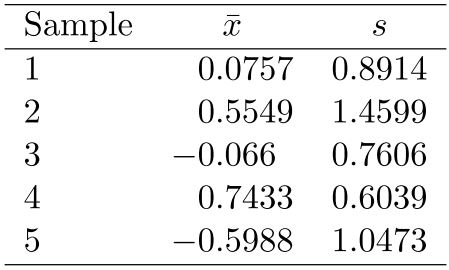
\includegraphics[scale=0.5]{Samples and observations.JPG}
\end{figure}

Note that all these samples each have different values since the observations vary from sample to sample, so does
any value computed from a sample. Capturing this uncertainty is a key component of \textbf{statistical analysis}.

\begin{tcolorbox}[breakable,colback=white]
\textbf{Statistic}: Any quantity calculated from sample data.
\end{tcolorbox}

Prior to obtaining the data, there is a level of uncertainty as to which value of the statistic will
occur. This uncertainty is modelled as a random variable thus \textbf{a statistic is a random
variable}. 

Since a statistic is a random variable, it has a probability distribution called the
\textbf{sampling distribution}. This distribution reflects how the statistic value varies across the
possible samples that could possibly be selected.

The \textbf{expected value} and \textbf{theoretical variance} of the sampling distribution will be important values.

%%%%%%%%%%%%%%%%%%%%%%%%%%%%%%%%%%%%%%%%%%%%%%%%%%%%%%%%%%%%%%%%%%%%%%%%%%%%%%%%%%%%%%%%%%%%%%%%%%%%%%%%%%
\section{Random samples}

The sampling distribution of a statistic depends on several factors:
\begin{itemize}
    \item Parent population size.
    \item Sample size.
    \item Sampling mechanism used.
\end{itemize}

\begin{tcolorbox}[breakable,colback=white]
\textbf{Random sample} (of size $n$ from a distribution with probability mass/density function
$f_X(x)$:  A set of independently and identically distributed random variables $X_1, X_2,\dots, X_n$ each with
mass/density function $f_X(x)$.
\end{tcolorbox}

\textbf{Example 1}: Consider the random variable X, with PMF: 
\begin{figure} [h!]
    \centering
    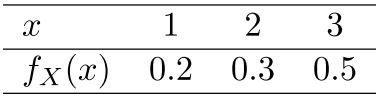
\includegraphics[scale=0.5]{Ex2.1 PMF.JPG}
\end{figure}

Two numbers $X_1$ and $X_2$ are drawn independently according to $f_X(x)$. Find the mean defined as
$\overline{X} = \frac{1}{n}\sum_{i=1}X_i$. The small range of $X$ makes it practical to consider
every pair $(X_1, X_2)$ and the corresponding mean.

Recall: 
\begin{itemize}
    \item \textbf{Independent}: Can compute $f_{X_1,X_2}(x1, x2) = P(X_1 = x_1 \cap X_2 = x_2)$.
\end{itemize}

Process: 
\begin{enumerate}
    \item Calculate the expected value of $\overline{X}$:
    \begin{align*}
        \overline{X} = \mu = 1(0.2) + 2(0.3) + 3(0.5) = 2.3
    \end{align*}
    \item Calculate the variance:
    \begin{align*}
        \text{Variance} = \frac{\sigma^2}{n} = \frac{\sum x^2p - \mu^2}{2} = 0.305
    \end{align*}
    \pagebreak
    \item Find the sampling distribution.
    \begin{figure} [h]
    \centering
    \begin{subfigure}{.5\textwidth}
      \centering
      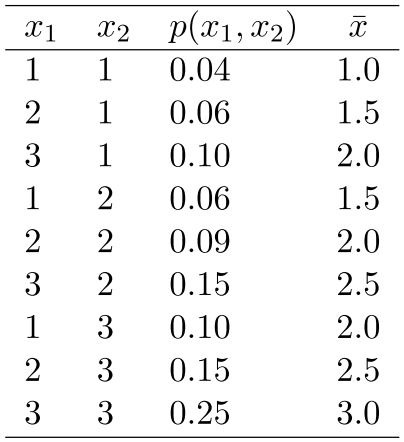
\includegraphics[scale=0.45]{sampling distr1.JPG}
      \caption{Each pair $(X1, X2)$ and the corresponding mean.}
      \label{fig:sub1}
    \end{subfigure}%
    \begin{subfigure}{.5\textwidth}
      \centering
      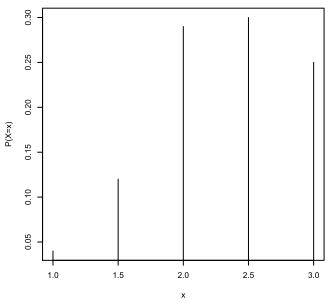
\includegraphics[scale=0.66]{sampling distr2.JPG}
      \caption{Sampling distribution}
      \label{fig:sub2}
    \end{subfigure}
 
    \end{figure}
\end{enumerate}

%%%%%%%%%%%%%%%%%%%%%%%%%%%%%%%%%%%%%%%%%%%%%%%%%%%%%%%%%%%%%%%%%%%%%%%%%%%%%%%%%%%%%%%%%%%%%%%%%%%%%%%%%%
\section{Distribution of sample mean}

Many important statistical procedures are concerned with making statements about the \textbf{population
mean} using the properties of the distribution of the \textbf{sample mean}.

If $X_1, X_2,\dots, X_n$ is a random sample from a population with mean $\mu$, variance $\sigma^2$
and sample mean $\overline{X}$:
\begin{itemize}
    \item Expected value $E[\overline{X}]$:
    \begin{tcolorbox}[breakable,colback=white]
        \begin{align*}
            E[\overline{X}] &= E\left(\frac{1}{n}\sum_{i=1}^n X_i\right) = E\left(\frac{1}{n}\sum_{i=1}^n E(X_i)\right) \\
            &= \frac{n \mu}{n} = \mu
        \end{align*}
    \end{tcolorbox}
    \item Variance $\text{Var}(\overline{X})$:
    \begin{tcolorbox}[breakable,colback=white]
    \begin{align*}
        \text{Var}(\overline{X}) &= \text{Var}\left(\frac{1}{n}\sum_{i=1}^n X_i\right) \\
        &= \frac{1}{n^2}\left(\sum_{i=1}^n \text{Var}(X_i)\right) \\
        &= \frac{n\sigma^2}{n^2} = \frac{\sigma^2}{n}
    \end{align*}
    \end{tcolorbox}
    \item Standard deviation:
    \begin{align*}
        \frac{\sigma}{\sqrt{n}}
    \end{align*}
    Commonly known as the \textbf{standard error} of the sample mean. This quantity decreases as the
    sample size increases.
\end{itemize}

A common relationship between parent normal distribution and the corresponding sampling
distributions for $\overline{X}$ \par
\begin{figure} [h!]
    \centering
    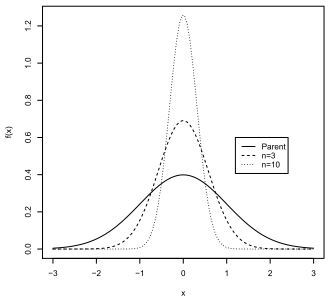
\includegraphics[scale=0.7]{parent vs sampling.JPG}
\end{figure}
is that as the sample size increases, the sampling distribution becomes increasingly concentrated
about its mean. When the parent population is normal, such that $X_1, X_2,\dots, X_n$ are
independent and share the identical base distribution $N(\mu, \sigma^2)$:
$$
    \overline{X} \sim N\left(\mu, \frac{\sigma^2}{n}\right) 
$$

\textbf{Example 1}: The total daily output of a titanium oxide facility is well modelled by a normal
distribution, with \textbf{mean $(\mu)$ $500$} tons, and \textbf{standard deviation $(\sigma)$ $50$}
tons. 

On $25$ randomly selected days per year the output is precisely measured and the sample mean
of the $25$ measurements is recorded as an annual $QC$ measure.

What is the probability that this sample mean is between $490$ and $510$?
\begin{enumerate}
    \item Denote the daily output as $X$:
    \begin{align*}
        X \sim N(500, 50^2) \; \text{ where sample size } n = 25
    \end{align*}
    \item Find $\overline{X} \sim N\left(\mu, \frac{\sigma^2}{n}\right)$ and the standardised version:
    \begin{align*}
        \overline{X} \sim N\left(500, \frac{50^2}{25}\right) \; \text{ and } \; Z = \frac{\overline{X}-500}{10} \sim N(0,1)
    \end{align*}
    \item Compute the probability:
    \begin{align*}
        P(490 \leq X \leq 510) = P(-1 \leq Z \leq 1) = \phi(1) - \phi(-1) = 0.682
    \end{align*}
\end{enumerate}

%%%%%%%%%%%%%%%%%%%%%%%%%%%%%%%%%%%%%%%%%%%%%%%%%%%%%%%%%%%%%%%%%%%%%%%%%%%%%%%%%%%%%%%%%%%%%%%%%%%%%%%%%%
\section{Central Limit Theorem}

\textbf{Statistical inference} is usually based on the sampling distribution of a statistic, but
there are few choices of parent distribution and statistic for which the sampling distribution can
be computed exactly. Most will require approximations.

Previously, the CLT can be used to approximate the sum of independent random variables from any distribution.
Using the properties of the normal distribution, the CLT can be extended to the sample mean:

\begin{tcolorbox}[breakable,colback=white]
    Given a random sample of size $n$ from a distribution with mean $\mu$ and variance $\sigma^2$,
    the distribution of $\overline{X}$ is \textbf{approximately} $N\left(\mu, \frac{\sigma^2}{n}\right)$ when
    $n$ is large enough.
\end{tcolorbox}

The quality of the approximation improves with increasing $n$.

%%%%%%%%%%%%%%%%%%%%%%%%%%%%%%%%%%%%%%%%%%%%%%%%%%%%%%%%%%%%%%%%%%%%%%%%%%%%%%%%%%%%%%%%%%%%%%%%%%%%%%%%%%
\section{Statistical analysis}

Probability theory provides the tools and models to reason about random experiments. When observing
a random variable $x$, the variable is treated as only one possible value of $X$. The objective of
statistical inference is to learn the aspects of the probability distribution which produced $x$, to
allow inferences to be drawn about the nature of the process under study.

The inferences drawn can be about various aspects. In this context, the inference drawn concerns with making
generalisations from the specific (the sample) to the general (the population). The notation used to represent the probability model for $x$:
\begin{align*}
    f(x|\theta)
\end{align*}
where:
\begin{itemize}
    \item $\theta$ - Parameters of the model i.e. $n$ and $p$ for a binomial random variable and $\lambda$ for an exponential.
\end{itemize}

The purpose of this notation is to make explicit that \textbf{the value of $\theta$ needs to be
known in order to evaluate the probability of a particular observation}. In all the previous
examples, the parameters and distribution were known and could easily evaluate probabilities such as $P(X >
3)$. 

Statistical problems often involve the reverse situation: \textbf{realisations} i.e. sample
observations for some unknown probability model are obtained. The goal is to estimate the values of
the model parameters. The questions involved will consider situations involving a known distribution
with unknown parameters. 

\begin{tcolorbox}[breakable,colback=white]
\textbf{Statistic}: A function that refers to a random sample.
\\
\\
\textbf{Estimator}: A statistic used to guess the value of some unknown parameter.
\end{tcolorbox}

Observing the sample $x_1, x_2,\dots, x_n$, two point of interest:
\begin{itemize}
    \item \textbf{Point estimation}: Estimating the value of unknown parameters.
    \item \textbf{Interval estimation}: Estimating an interval that contains the unknown parameters with high probability.
\end{itemize}

%%%%%%%%%%%%%%%%%%%%%%%%%%%%%%%%%%%%%%%%%%%%%%%%%%%%%%%%%%%%%%%%%%%%%%%%%%%%%%%%%%%%%%%%%%%%%%%%%%%%%%%%%%
\subsection{Point estimation}

Suppose it is of interest the true average lifetime of a specific type of spark plug i.e. population
mean value $\mu$. Obtain a random sample $x_1, x_2,\dots, x_9$ of $n = 9$ spark plugs to make an
observation. The sample mean $\overline{x}$ can be used to make statements about $\mu$. Other statistics
can also be used to make related statements e.g. the sample variance $s^2$ provides information
about the population variance $\sigma^2$.

\begin{tcolorbox}[breakable,colback=white]
    Sample realisations and statistics are usually denoted with Roman symbols, like $\overline{x}$
    and $s$, whereas unknown population parameters are denoted with Greek symbols, like $\mu$ and $\theta$.
\end{tcolorbox}

The objective of point estimation is to use a sample of data to provide a guess of an unknown
population parameter. 

\begin{tcolorbox}[breakable,colback=white]
\textbf{Point estimate} (of an unknown population parameter $\theta$): A single number which
represents the “best guess” of $\theta$ that arises from selecting a suitable statistic and computing
its value from a sample.
\end{tcolorbox}

The selected statistic is called a \textbf{point estimator} for $\theta$ denoted by $\hat{\theta}$.

\textbf{Example 1}: A chemical plant produces a compound that contains a particular component B. A
random sample of size $n = 11$ batches of this compound was obtained to measure the percentages of component
B in each. The results are as follows:
\begin{align*}
    5.3, 4.9, 6.2, 5.7, 4.8, 5.4, 6.1, 6.3, 5.6, 5.5, 7.2
\end{align*}
Assuming that the normal distribution with mean $\mu$ provides a plausible model for the percentage
of B and that this distribution is symmetric, $\mu$ can be estimated several ways:
\begin{itemize}
    \item \textbf{Sample mean}: 
    \begin{align*}
        \overline{x} = \frac{1}{n} \sum_{i=1}^{11} x_i = 5.72
    \end{align*}
    \item \textbf{Sample median}:
    \begin{align*}
        \tilde{x} = \frac{(x_5+x_6)}{2} = 5.6
    \end{align*}
    \item \textbf{Midpoint between the extremes}:
    \begin{align*}
        \frac{x_11 + x_12}{2} = 6
    \end{align*}
\end{itemize}
The quality cannot be directly assessed since the value of the parameter is unknown, thus
estimations have to be selected among estimators using other criteria.

%%%%%%%%%%%%%%%%%%%%%%%%%%%%%%%%%%%%%%%%%%%%%%%%%%%%%%%%%%%%%%%%%%%%%%%%%%%%%%%%%%%%%%%%%%%%%%%%%%%%%%%%%%
\subsection{Properties of estimators}

Recall that statistics are functions of random samples and all have a sampling distribution. The
sampling distribution provides a description of the random behaviour of the statistic thus can be
used to determine choice of estimator used.

Two criteria that sometimes lead to accurate estimators are:
\begin{itemize}
    \item Unbiasedness
    \item Minimum variance
\end{itemize}

%%%%%%%%%%%%%%%%%%%%%%%%%%%%%%%%%%%%%%%%%%%%%%%%%%%%%%%%%%%%%%%%%%%%%%%%%%%%%%%%%%%%%%%%%%%%%%%%%%%%%%%%%%
\subsubsection{Estimator bias}

Given a point estimator $\hat{\theta}$:
\begin{tcolorbox}[breakable,colback=white]
\textbf{Bias} (of $\hat{\theta}$): The difference between expected value \textbf{of estimator}
and a given value $\theta$:
$$
    \text{Bias of } \theta = E(\hat{\theta}) - \theta
$$

A point estimator $\hat{\theta}$ is an \textbf{unbiased estimator} of $\theta$ if $E(\hat{\theta}) = \theta$,
for all $\theta$. The bias for an unbiased estimator is $0$.
\end{tcolorbox}

The definition of an unbiased estimator states that the sampling distribution of an unbiased
estimator has a expected value equal to the population value $\theta$. Thus, if the experiment is repeated an
infinite number of times, on average an unbiased estimator would yield the correct answer.

If the parent population is known, the bias of an estimator $\hat{\theta}$ can be found even if
$\theta$ is unknown.

\textbf{Example 1}: Components of a certain type are either operable or defective. It is of interest
in the random variable $X$ that counts the number of defective components in a batch of $50$ components.

This is a binomial experiment. A batch is randomly selected and the components tested. $X = 3$
defective is found. Use different ways techniques to estimate the unknown probability that a
component is defective denoted $p$.

Estimate 1: The basic probability:
\begin{align*}
    \hat{p} &= \frac{X}{n} \\
    &= \frac{3}{50} \\
    &= 0.06
\end{align*}

Estimate 2: Finding the bias and determining a better estimate:
\begin{enumerate}
    \item Find the expected value of the estimator:
    \begin{align*}
        E(\hat{p}) = E\left(\frac{X}{n}\right) = \frac{E(x)}{n} = \frac{np}{n} = p
    \end{align*}
    \item The estimator is an \textbf{unbiased estimator} of $p$.
\end{enumerate}

%%%%%%%%%%%%%%%%%%%%%%%%%%%%%%%%%%%%%%%%%%%%%%%%%%%%%%%%%%%%%%%%%%%%%%%%%%%%%%%%%%%%%%%%%%%%%%%%%%%%%%%%%%
\subsubsection{Minimum variance estimators}

When selecting among unbiased estimators of $\theta$, the estimator with \textbf{minimum variance}
is chosen since the minimum variance estimator has the most concentrated distribution. 

There is a special term for this: \textbf{Minimum variance unbiased estimator} (MVUE) of $\theta$.

%%%%%%%%%%%%%%%%%%%%%%%%%%%%%%%%%%%%%%%%%%%%%%%%%%%%%%%%%%%%%%%%%%%%%%%%%%%%%%%%%%%%%%%%%%%%%%%%%%%%%%%%%%
\subsubsection{Mean square error}

While the MVUE is desirable, it is often possible to obtain an estimator with small bias, but
appreciably smaller variance.

For this reason, choose the estimator which minimises the \textbf{mean squared error (MSE)} defined:
\begin{align*}
    MSE_\theta (\hat{\theta}) = E[(\hat{\theta}-\theta)^2] = \text{Var}(\hat{\theta}) + \left(\text{Bias}_\theta(\hat{\theta}) \right)^2
\end{align*}

%%%%%%%%%%%%%%%%%%%%%%%%%%%%%%%%%%%%%%%%%%%%%%%%%%%%%%%%%%%%%%%%%%%%%%%%%%%%%%%%%%%%%%%%%%%%%%%%%%%%%%%%%%
\section{Standard errors}

The standard error of the sample mean i.e. the standard deviation of the sampling distribution of the
mean can be extended to any estimator.

\begin{tcolorbox}[breakable,colback=white]
\textbf{Standard error} of estimator $\theta$ - $\sigma_{\hat{\theta}}$: The standard deviation of estimator:
\begin{align*}
    \text{Standard error} = \sqrt{\text{Var}(\hat{\theta})}
\end{align*} 
\end{tcolorbox}

Sometimes, the standard error will depend on unknown parameters that must be estimated. In this
case, the \textbf{estimated standard error} of the estimator $\hat{\sigma}_{\hat{\theta}}$ is used.

\textbf{Example 1:} \textbf{Example 1}: A chemical plant produces a compound that contains a particular component B. A
random sample of size $n = 11$ batches of this compound was obtained to measure the percentages of component
B in each. The results are as follows:
\begin{align*}
    5.3, 4.9, 6.2, 5.7, 4.8, 5.4, 6.1, 6.3, 5.6, 5.5, 7.2
\end{align*}
Assuming that the normal distribution with unknown mean $\mu$ and unknown variance $\sigma^2$:
$$
    \overline{X} \sim N\left(\mu, \frac{\sigma^2}{n}\right)
$$
find the estimated standard error.
\begin{align*}
    s^2 = \frac{1}{n-1} \sum_{x=1}^n (x_i - \overline{x})^2 = 0.476
\end{align*}
Estimated error is:
\begin{align*}
    s_{\overline{X}} = 0.2
\end{align*}

%%%%%%%%%%%%%%%%%%%%%%%%%%%%%%%%%%%%%%%%%%%%%%%%%%%%%%%%%%%%%%%%%%%%%%%%%%%%%%%%%%%%%%%%%%%%%%%%%%%%%%%%%%
\section{Point estimation methods}

The previous section listed the desirable characteristics of estimators without specifying how to
construct estimators. There are a number of methods are available for automatically constructing
estimators:
\begin{itemize}
    \item Method of moments
    \item Least squares
    \item Maximum likelihood (ML)
\end{itemize}

In general, ML estimation is preferred in statistics because of desirable theoretical properties,
although in realistic contexts, it sometimes require significant computation.

%%%%%%%%%%%%%%%%%%%%%%%%%%%%%%%%%%%%%%%%%%%%%%%%%%%%%%%%%%%%%%%%%%%%%%%%%%%%%%%%%%%%%%%%%%%%%%%%%%%%%%%%%%
\subsection{Method of moments}

The method of moments attempts to equate sample characteristics with corresponding population
theoretical values. Its estimators are the solutions to such equations that satisfies the ideal
characteristics.

Consider a random sample $X_1, X_2,\dots, X_n$ from PDF or PMF $f(x)$.  Recall that the $k^{th}$
moment of $X$ is defined $m_k = E(X^k)$. The \textbf{sample moments} - sample equivalent of
theoretical moments are defined:
$$
    \frac{1}{n} \sum_{i=1}^n X_i^k \; \text{for } k = 1,2,\dots
$$

The process gets complicated when there are more parameters that need to be estimated.

Some common theoretical moments are:
\begin{itemize}
    \item First theoretical moment $E(X)=\mu$ and corresponding sample moment is
    $\frac{1}{n}\sum_{i=1}^n X_i$
    \item Second theoretical moment $E[X^2]$ and corresponding sample moment is
    $\frac{1}{n}\sum_{i=1}^n X_i^2$
\end{itemize}

\textbf{Example 1}: 

%%%%%%%%%%%%%%%%%%%%%%%%%%%%%%%%%%%%%%%%%%%%%%%%%%%%%%%%%%%%%%%%%%%%%%%%%%%%%%%%%%%%%%%%%%%%%%%%%%%%%%%%%%
\subsection{Maximum likelihood (ML)}

Maximum-likelihood estimation is usually the recommended approach, since the estimators have
desirable properties. This approach is built around the joint probability or density of the
collection of random variables in a sample.

\begin{tcolorbox}[breakable,colback=white]
Given same $X_1,X_2,...,X_n$ with joint density or PMF:
$$
    L(\theta) = f(X_1 = x_1, \dots , X_n = x_n|\theta)
$$
where $\theta$ refers to unknown parameters.
\end{tcolorbox}

\textbf{Likelihood function}: The joint probability is regarded as a function of $\theta$. The value
of $\theta$ that maximises the likelihood function is known as the \textbf{maximum-likelihood
estimators} (MLE) of $\theta$. The estimates evaluated for observed values yield
\textbf{maximum-likelihood estimates}.

The maximum-likelihood estimators give the values of $\theta$ that agree mostly closely with the
observed data. Due to the property of independence, the joint density/mass function of a random
sample decomposes into a product of the marginal density/mass functions.

\begin{tcolorbox}[breakable,colback=white]
General ML process:
\begin{enumerate}
    \item Write and simplify the likelihood.
    \item Take logs.
    \item Differentiate and equate the resulting equations with $0$ and solve. 
    \item Examine the second derivatives.
\end{enumerate}
\end{tcolorbox}

%%%%%%%%%%%%%%%%%%%%%%%%%%%%%%%%%%%%%%%%%%%%%%%%%%%%%%%%%%%%%%%%%%%%%%%%%%%%%%%%%%%%%%%%%%%%%%%%%%%%%%%%%%
\end{document}